\section{Event Selection}\label{section:star_event_selection}
Events were selected from those passing the SDT trigger condition. In order to remove events having poor quality and background the following conditions were required:
\begin{enumerate}
	\item Trigger signals in exactly two stations of one arm of \ac{RP} system,
	\item Any trigger signal in small BBC tiles on the opposite side of the STAR central detector to the~triggered RP station,
	\item Exactly one proton track in the above RP stations with $0.02 < \xi < 0.2$ and $0.04 < -t < 0.16$~GeV$^{2}$/c$^{2}$. 
	\item Exactly one primary vertex with TPC tracks matched with hits in TOF (later in the~text such vertex  is refered as a TOF vertex),
	\item TPC vertex  within $|V_z|<80$~cm - events with vertices away from the IP have low acceptance for the central and forward tracks,
	\item At least two but no more than eight primary TPC tracks, $2\leq n_{\textrm{sel}}\leq 8$, matched with hits in TOF and satisfying the selection criteria described in Sec.~\ref{section:star_track_selection},
	\item If there are exactly two primary tracks satisfying above criteria and exactly two global tracks used in vertex reconstruction (Sec.~\ref{section:star_vertex}), the longitudinal distance between these global tracks should be smaller than $2$~cm, $|\Delta z_0|<2$~cm, due to small ($<20\%$) vertex reconstruction efficiency for tracks with $|\Delta z_0|>2$~cm (as described in Sec.~\ref{section:star_vertex}).
\end{enumerate}
Figure~\ref{fig:vertexSTAR} shows the multiplicity of TOF vertices (left) and the $z$-position of primary vertex in a~single TOF vertex events (right). Data are compared to embedded PYTHIA~8 SD sample. These distributions are not significantly process-dependent, therefore, contributions from other processes are not included in these plots.

\begin{figure}[h!]
	\centering
	\includegraphics[width=.49\textwidth, page=10]{chapters/chrgSTAR/img/selection/SDT.pdf}
	\includegraphics[width=.49\textwidth, page=5]{chapters/chrgSTAR/img/selection/SDT.pdf}
	\caption{(left) Primary vertex multiplicity  and  (right) the $z$-position of primary vertex in a single TOF vertex events before applying  the~cut on the~quantity shown. Blue lines indicate regions accepted in the analysis.}
	\label{fig:vertexSTAR}
\end{figure}

\FloatBarrier